\documentclass[aspectratio=169,11pt]{beamer}

\usepackage[utf8]{inputenc}
\usepackage[T1]{fontenc}
\usepackage{lmodern}
\usepackage{xcolor}
\usepackage{tcolorbox}
\tcbuselibrary{skins, breakable}

\usepackage{tikz}
\usetikzlibrary{positioning, shapes.geometric, shapes.symbols, arrows.meta, calc, fit, backgrounds, shadows.blur}

\definecolor{swTeal}{HTML}{2A9D8F}
\definecolor{swTealDark}{HTML}{258B7F}
\definecolor{swTealLight}{HTML}{E6F4F1}
\definecolor{swAmber}{HTML}{E9C46A}
\definecolor{swAmberLight}{HTML}{FBF4DC}
\definecolor{swSlate}{HTML}{598392}
\definecolor{swInk}{HTML}{1F2933}
\definecolor{swMute}{HTML}{6B7280}
\definecolor{swBg}{HTML}{F7F9FA}
\definecolor{swRed}{HTML}{C03A3A}
\definecolor{swRedLight}{HTML}{FFF5F5}
\definecolor{swBlue}{HTML}{0078D4}
\definecolor{swBlueLight}{HTML}{F0F7FF}
\definecolor{swGreen}{HTML}{2F9E44}
\definecolor{swGreenLight}{HTML}{ECFDF3}

% Hyperref loaded last so it can hook into the page model. Link colours
% picked from the SiliconWit palette so they read as deliberate UI.
\usepackage{hyperref}
\hypersetup{
  colorlinks=true,
  linkcolor=swTealDark,
  urlcolor=swTealDark,
  citecolor=swTealDark,
  filecolor=swTealDark,
  pdftitle={Install SiliconWit Seal},
  pdfsubject={OpenPGP file encryption for everyone},
  pdfauthor={SiliconWit},
  pdfkeywords={OpenPGP, GnuPG, PGP, Seal, SiliconWit, encryption, install},
  bookmarksopen=true,
  bookmarksnumbered=true,
  pdfstartview={FitH}
}

\usetheme{default}
\useinnertheme{default}
\useoutertheme{default}
\setbeamertemplate{navigation symbols}{}

\setbeamercolor{normal text}{fg=swInk, bg=white}
\setbeamercolor{frametitle}{fg=swTealDark, bg=white}
\setbeamercolor{title}{fg=swTealDark}
\setbeamercolor{subtitle}{fg=swSlate}
\setbeamercolor{author}{fg=swMute}
\setbeamercolor{itemize item}{fg=swTeal}
\setbeamercolor{itemize subitem}{fg=swAmber}
\setbeamercolor{structure}{fg=swTeal}

\setbeamerfont{frametitle}{size=\Large, series=\bfseries}
\setbeamerfont{title}{size=\Huge, series=\bfseries}
\setbeamerfont{subtitle}{size=\large}

\setbeamertemplate{frametitle}{%
  \vspace{0.4em}%
  \begin{beamercolorbox}[wd=\paperwidth, leftskip=0.6cm, rightskip=0.6cm]{frametitle}%
    \insertframetitle%
    \vskip2pt%
    {\color{swAmber}\rule{2.2em}{2pt}}%
  \end{beamercolorbox}%
  \vspace{0.2em}%
}

\setbeamertemplate{itemize item}{\textcolor{swTeal}{\textbullet}}
\setbeamertemplate{itemize subitem}{\textcolor{swAmber}{\textendash}}

% Page X of Y footer. The deck title sits on the left, the page counter
% on the right. Plain frames (the title and closing slide) skip this
% automatically because beamer suppresses the footline on [plain] frames.
\setbeamercolor{footline}{fg=swMute, bg=white}
\setbeamertemplate{footline}{%
  \leavevmode%
  \hbox{%
    \begin{beamercolorbox}[wd=\paperwidth, ht=2.6ex, dp=1.2ex,
        leftskip=0.6cm, rightskip=0.6cm]{footline}%
      \tiny%
      \textcolor{swMute}{Install SiliconWit Seal}%
      \hfill%
      \textcolor{swMute}{\insertframenumber\ of \inserttotalframenumber}%
    \end{beamercolorbox}%
  }%
  \vspace{2pt}%
}

\newtcolorbox{cmdbox}{
  enhanced, breakable,
  colback=swBg, colframe=swSlate!40,
  boxrule=0.4pt, arc=2pt,
  left=8pt, right=8pt, top=4pt, bottom=4pt,
  fontupper=\ttfamily\small
}

\newtcolorbox{notebox}[1][Note]{
  enhanced,
  colback=swAmber!12, colframe=swAmber,
  boxrule=0.6pt, arc=2pt,
  left=8pt, right=8pt, top=4pt, bottom=4pt,
  title={\bfseries #1},
  coltitle=swTealDark, colbacktitle=swAmber!30,
  fonttitle=\small, fontupper=\small
}

% Common TikZ styles. Defining them once keeps each diagram concise and
% visually consistent across slides.
\tikzset{
  card/.style={
    rectangle, rounded corners=6pt,
    draw=#1, line width=0.7pt,
    fill=#1!8,
    inner sep=8pt,
    minimum width=3.2cm, minimum height=1.6cm,
    align=center,
    font=\small
  },
  wizardstep/.style={
    rectangle, rounded corners=4pt,
    draw=swTeal, line width=0.5pt,
    fill=swTealLight,
    inner sep=5pt,
    minimum width=2.2cm, minimum height=1.0cm,
    align=center, font=\footnotesize
  },
  arrow/.style={
    -{Stealth[length=2.6mm, width=2.0mm]},
    swSlate, line width=0.7pt
  },
  thickarrow/.style={
    -{Stealth[length=3.6mm, width=2.8mm]},
    swTealDark, line width=1.0pt
  },
  folder/.style={
    rectangle, rounded corners=3pt,
    draw=swSlate!60, line width=0.4pt,
    fill=swBg,
    inner sep=4pt,
    minimum width=3.0cm, minimum height=0.7cm,
    align=left, font=\footnotesize\ttfamily
  },
  legend/.style={font=\scriptsize\itshape, swMute}
}

\newcommand{\releasesurl}{https://github.com/SiliconWit/siwit-seal-releases/releases}
\newcommand{\docsurl}{https://siliconwit.github.io/siwit-seal-releases/}
\newcommand{\winmirror}{https://drive.google.com/file/d/1\_sCuSeqJO8JbBs8dWMn0VtlgerIXMrI3/view?usp=sharing}

\title{Install SiliconWit Seal}
\subtitle{OpenPGP file encryption for everyone}
\author{SiliconWit}
\date{}

\begin{document}

% ===== Slide 1: title =====================================================
\begin{frame}[plain]
  \vspace*{1.2cm}
  \begin{center}
    {\color{swTealDark}\rule{3em}{4pt}}\\[1.2em]
    {\usebeamerfont{title}\usebeamercolor[fg]{title}\inserttitle}\\[0.4em]
    {\usebeamerfont{subtitle}\usebeamercolor[fg]{subtitle}\insertsubtitle}\\[2em]
    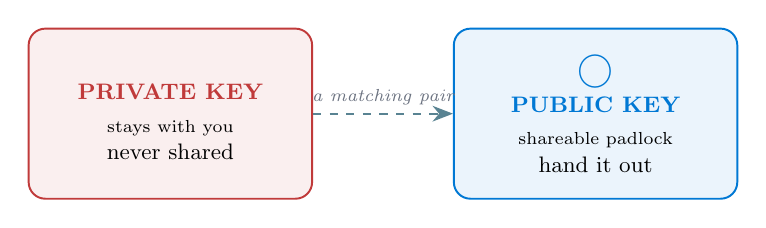
\begin{tikzpicture}[scale=0.9, transform shape]
      \node[card=swRed, minimum width=4cm, minimum height=2.4cm] (priv) at (0,0)
        {\textcolor{swRed}{\Large $\blacksquare$}\\[2pt]
         {\color{swRed}\bfseries PRIVATE KEY}\\[2pt]
         \scriptsize stays with you\\never shared};
      \node[card=swBlue, minimum width=4cm, minimum height=2.4cm] (pub) at (6,0)
        {\textcolor{swBlue}{\Large $\bigcirc$}\\[2pt]
         {\color{swBlue}\bfseries PUBLIC KEY}\\[2pt]
         \scriptsize shareable padlock\\hand it out};
      \draw[arrow, dashed] (priv.east) -- node[above, legend]{a matching pair} (pub.west);
    \end{tikzpicture}\\[1.6em]
    {\small\href{\docsurl}{siliconwit.github.io/siwit-seal-releases}}
  \end{center}
\end{frame}

% ===== Slide 2: what you are installing ==================================
\begin{frame}{What you are installing}
  \begin{columns}[T,onlytextwidth]
    \begin{column}{0.56\textwidth}
      \begin{itemize}
        \item Desktop app for encrypting and decrypting files using OpenPGP.
        \item Drag a file in. Get a \texttt{.gpg} you can email.
        \item Drag a \texttt{.gpg} in. Get the contents back.
        \item GnuPG is bundled. No separate install. No command line.
        \item Output is standard OpenPGP (RFC 4880). Recipients can open it with Kleopatra, GPG Suite, Thunderbird, Mailvelope, or any other OpenPGP tool. They do \textbf{not} need to install Seal.
      \end{itemize}
    \end{column}
    \begin{column}{0.42\textwidth}
      \centering
      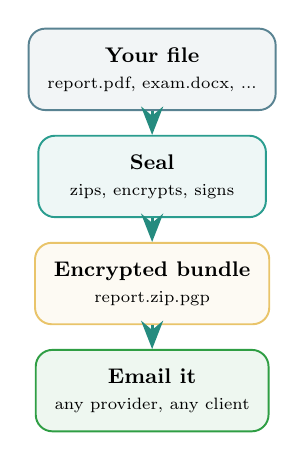
\begin{tikzpicture}[scale=0.85, transform shape]
        \node[card=swSlate, minimum width=3.4cm, minimum height=1.2cm] (file) at (0,2.6) {\textbf{Your file}\\\scriptsize report.pdf, exam.docx, ...};
        \node[card=swTeal, minimum width=3.4cm, minimum height=1.2cm] (seal) at (0,1.0) {\textbf{Seal}\\\scriptsize zips, encrypts, signs};
        \node[card=swAmber, minimum width=3.4cm, minimum height=1.2cm] (out) at (0,-0.6) {\textbf{Encrypted bundle}\\\scriptsize report.zip.pgp};
        \node[card=swGreen, minimum width=3.4cm, minimum height=1.2cm] (mail) at (0,-2.2) {\textbf{Email it}\\\scriptsize any provider, any client};
        \draw[thickarrow] (file.south) -- (seal.north);
        \draw[thickarrow] (seal.south) -- (out.north);
        \draw[thickarrow] (out.south) -- (mail.north);
      \end{tikzpicture}
    \end{column}
  \end{columns}
\end{frame}

% ===== Slide 3: key concept diagram (private vs public) ==================
\begin{frame}{The one idea: padlock and key}
  \begin{center}
    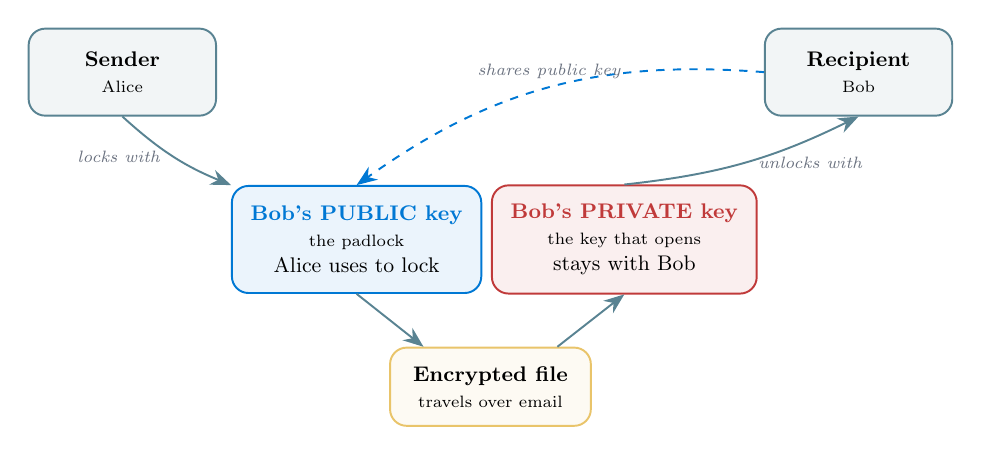
\begin{tikzpicture}[scale=0.85, transform shape]
      % Sender side
      \node[card=swSlate, minimum width=2.8cm, minimum height=1.3cm] (sender) at (-5.5, 1.5) {\textbf{Sender}\\\scriptsize Alice};
      % Recipient side
      \node[card=swSlate, minimum width=2.8cm, minimum height=1.3cm] (recipient) at (5.5, 1.5) {\textbf{Recipient}\\\scriptsize Bob};
      % Public key (Bob's, held by Alice)
      \node[card=swBlue, minimum width=3.0cm, minimum height=1.6cm] (pub) at (-2.0, -1.0) {{\color{swBlue}\bfseries Bob's PUBLIC key}\\\scriptsize the padlock\\Alice uses to lock};
      % Private key (Bob's)
      \node[card=swRed, minimum width=3.0cm, minimum height=1.6cm] (priv) at (2.0, -1.0) {{\color{swRed}\bfseries Bob's PRIVATE key}\\\scriptsize the key that opens\\stays with Bob};
      % File flow
      \node[card=swAmber, minimum width=3.0cm, minimum height=1.0cm] (file) at (0, -3.2) {\textbf{Encrypted file}\\\scriptsize travels over email};
      % Arrows: Bob shares public key, Alice locks, file travels, Bob unlocks
      \draw[arrow, dashed, swBlue] (recipient.west) to[bend right=20] node[above, legend, align=center]{shares public key} (pub.north);
      \draw[arrow, swSlate] (sender.south) to[bend right=10] node[left, legend, xshift=-2pt]{locks with} (pub.north west);
      \draw[arrow] (pub.south) -- ($(file.north)+(-1.0,0)$);
      \draw[arrow] ($(file.north)+(1.0,0)$) -- (priv.south);
      \draw[arrow, swSlate] (priv.north) to[bend right=10] node[right, legend, xshift=2pt]{unlocks with} (recipient.south);
    \end{tikzpicture}\\[0.4em]
    \small Alice never sees Bob's private key. Only Bob can open the file.
  \end{center}
\end{frame}

% ===== Slide 4: get the installer ========================================
\begin{frame}{Get the installer}
  \begin{itemize}
    \item Open the official Releases page (click the link in the PDF):
  \end{itemize}
  \begin{cmdbox}
\href{\releasesurl}{github.com/SiliconWit/siwit-seal-releases/releases}
  \end{cmdbox}
  \begin{itemize}
    \item Pick the asset for your operating system: \texttt{.deb} for Linux, \texttt{.msi} for Windows, \texttt{.dmg} for macOS.
    \item Optional but recommended: verify the SHA-256 against the published checksum.
  \end{itemize}
  \begin{cmdbox}
sha256sum -c siwit-seal-<version>.sha256                  \# Linux, macOS\\
Get-FileHash siwit-seal-<version>.msi -Algorithm SHA256   \# Windows PS
  \end{cmdbox}
\end{frame}

% ===== Slide 5: Windows ==================================================
\begin{frame}{Windows}
  \textbf{Tested on Windows 10 (1909+) and Windows 11.}
  \begin{enumerate}
    \item Download \texttt{siwit-seal-<version>-win-x64.msi} from \href{\releasesurl}{GitHub Releases} or the \href{\winmirror}{Google Drive mirror} (byte-identical).
    \item Double-click the \texttt{.msi}. Follow the installer prompts.
    \item Launch \textbf{SiliconWit Seal} from the Start menu.
  \end{enumerate}
  \begin{notebox}[Expected warnings, normal for new open-source software]
    Browser \emph{not commonly downloaded}: click \textbf{Keep}.\\
    Google Drive \emph{can't scan for viruses}: click \textbf{Download anyway}.\\
    Windows SmartScreen: click \textbf{More info}, then \textbf{Run anyway}.\\
    UAC prompt: click \textbf{Yes}.
  \end{notebox}
  \vspace{0.2em}
  \small\textcolor{swMute}{Keyring: \texttt{\%APPDATA\%\textbackslash Seal\textbackslash}. Visible files: \texttt{Documents\textbackslash SILICONWIT-SEAL\textbackslash}.}
\end{frame}

% ===== Slide 6: Linux ====================================================
\begin{frame}{Linux (Debian, Ubuntu, Mint)}
  \textbf{Tested on Ubuntu 22.04+, Debian 12+, Linux Mint 21+.}
  \begin{enumerate}
    \item Download \texttt{siwit-seal\_<version>\_amd64.deb} from \href{\releasesurl}{GitHub Releases}.
    \item Install with \texttt{apt} so dependencies resolve automatically (the leading \texttt{./} is required):
  \end{enumerate}
  \begin{cmdbox}
sudo apt install ./siwit-seal\_<version>\_amd64.deb
  \end{cmdbox}
  \begin{enumerate}
    \setcounter{enumi}{2}
    \item Launch from the applications menu (search \emph{SiliconWit Seal}), or run \texttt{siwit-seal} in a terminal.
  \end{enumerate}
  \vspace{0.4em}
  \small\textcolor{swMute}{Keyring: \texttt{\textasciitilde/.local/share/Seal/}. Visible files: \texttt{\textasciitilde/Documents/SILICONWIT-SEAL/}.}
\end{frame}

% ===== Slide 7: macOS ====================================================
\begin{frame}{macOS}
  \textbf{Coming soon. Apple Silicon and Intel, macOS 12+.}
  \begin{enumerate}
    \item Download \texttt{SiliconWit-Seal-<version>.dmg} from \href{\releasesurl}{Releases}.
    \item Open the \texttt{.dmg}. Drag \textbf{SiliconWit Seal} into \texttt{Applications}.
    \item First launch: right-click, then \textbf{Open}, then confirm.
  \end{enumerate}
  \vspace{0.4em}
  \begin{notebox}[Why right-click on first launch]
    The build is not yet notarized, so Gatekeeper holds it on first run.
    Right-click then \textbf{Open} is the supported override. After the
    first launch, double-click works normally.
  \end{notebox}
  \vspace{0.2em}
  \small\textcolor{swMute}{Keyring: \texttt{\textasciitilde/Library/Application Support/Seal/}.}
\end{frame}

% ===== Slide 8: first-run wizard diagram =================================
\begin{frame}{First run: the setup wizard}
  \begin{center}
    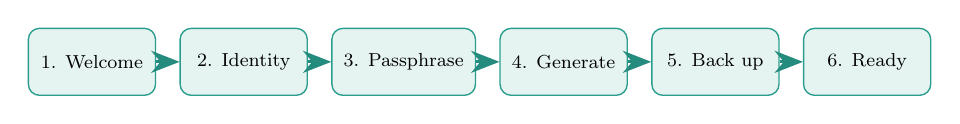
\begin{tikzpicture}[node distance=0.35cm, scale=0.85, transform shape]
      \node[wizardstep, minimum width=1.9cm] (s1) {1. Welcome};
      \node[wizardstep, minimum width=1.9cm, right=of s1] (s2) {2. Identity};
      \node[wizardstep, minimum width=1.9cm, right=of s2] (s3) {3. Passphrase};
      \node[wizardstep, minimum width=1.9cm, right=of s3] (s4) {4. Generate};
      \node[wizardstep, minimum width=1.9cm, right=of s4] (s5) {5. Back up};
      \node[wizardstep, minimum width=1.9cm, right=of s5] (s6) {6. Ready};
      \draw[thickarrow] (s1) -- (s2);
      \draw[thickarrow] (s2) -- (s3);
      \draw[thickarrow] (s3) -- (s4);
      \draw[thickarrow] (s4) -- (s5);
      \draw[thickarrow] (s5) -- (s6);
    \end{tikzpicture}
  \end{center}
  \vspace{0.4em}
  \begin{columns}[T,onlytextwidth]
    \begin{column}{0.48\textwidth}
      \footnotesize
      \begin{itemize}
        \item \textbf{1 Welcome.} Public key vs. private key explained side by side.
        \item \textbf{2 Identity.} Real name and email for your public key.
        \item \textbf{3 Passphrase.} Protects your private key. No recovery if lost.
      \end{itemize}
    \end{column}
    \begin{column}{0.48\textwidth}
      \footnotesize
      \begin{itemize}
        \item \textbf{4 Generate.} 4096-bit RSA, up to a minute.
        \item \textbf{5 Back up.} Save the \textbf{private-key backup} and the \textbf{revocation certificate} somewhere safe.
        \item \textbf{6 Ready.} Fingerprint shown so you can verify with contacts.
      \end{itemize}
    \end{column}
  \end{columns}
  \vspace{0.2em}
  \begin{notebox}[Keep both backups safe]
    Lose the passphrase and the backup, and old files cannot be opened.
    The revocation certificate is the only way to publicly invalidate a lost
    or compromised key later. Save both \textbf{before} encrypting real material.
  \end{notebox}
\end{frame}

% ===== Slide 9: send flow diagram ========================================
\begin{frame}{Send: how a file becomes a bundle}
  \begin{center}
    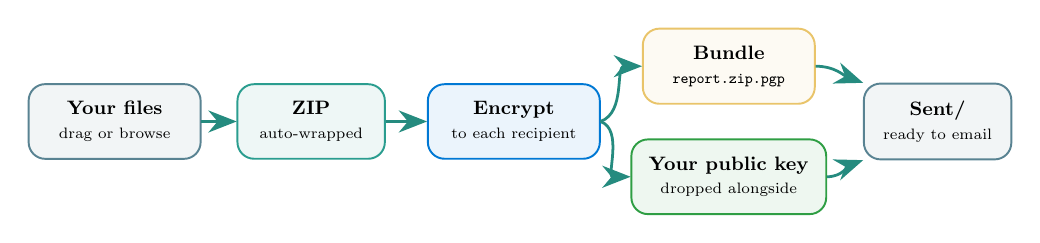
\begin{tikzpicture}[scale=0.78, transform shape]
      \node[card=swSlate, minimum width=2.8cm, minimum height=1.2cm] (files) at (-6.0, 0) {\textbf{Your files}\\\scriptsize drag or browse};
      \node[card=swTeal, minimum width=2.4cm, minimum height=1.2cm] (zip) at (-2.8, 0) {\textbf{ZIP}\\\scriptsize auto-wrapped};
      \node[card=swBlue, minimum width=2.8cm, minimum height=1.2cm] (enc) at (0.5, 0) {\textbf{Encrypt}\\\scriptsize to each recipient};
      \node[card=swAmber, minimum width=2.8cm, minimum height=1.2cm] (bundle) at (4.0, 0.9) {\textbf{Bundle}\\\scriptsize \texttt{report.zip.pgp}};
      \node[card=swGreen, minimum width=2.8cm, minimum height=1.2cm] (pubdrop) at (4.0, -0.9) {\textbf{Your public key}\\\scriptsize dropped alongside};
      \node[card=swSlate, minimum width=2.4cm, minimum height=1.2cm] (sent) at (7.4, 0) {\textbf{Sent/}\\\scriptsize ready to email};
      \draw[thickarrow] (files) -- (zip);
      \draw[thickarrow] (zip) -- (enc);
      \draw[thickarrow] (enc.east) to[out=20, in=180] (bundle.west);
      \draw[thickarrow] (enc.east) to[out=-20, in=180] (pubdrop.west);
      \draw[thickarrow] (bundle.east) to[out=0, in=160] (sent.north west);
      \draw[thickarrow] (pubdrop.east) to[out=0, in=-160] (sent.south west);
    \end{tikzpicture}\\[0.4em]
    \small Seal saves both files in \texttt{Documents/SILICONWIT-SEAL/Sent/}. Attach both to your email.
  \end{center}
\end{frame}

% ===== Slide 10: receive flow diagram ====================================
\begin{frame}{Receive: how a bundle becomes files}
  \begin{center}
    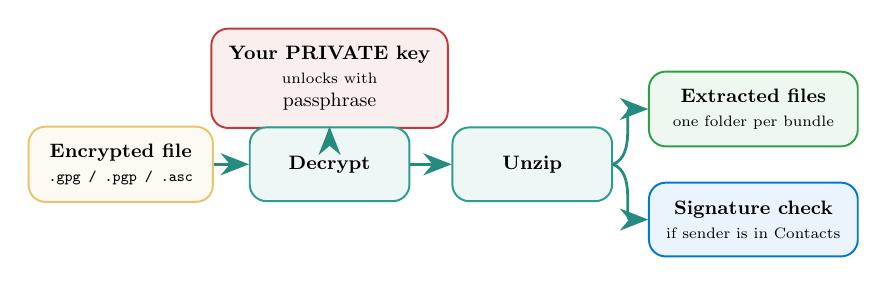
\begin{tikzpicture}[scale=0.78, transform shape]
      \node[card=swAmber, minimum width=3.0cm, minimum height=1.2cm] (in) at (-6.0, 0) {\textbf{Encrypted file}\\\scriptsize \texttt{.gpg / .pgp / .asc}};
      \node[card=swRed, minimum width=2.6cm, minimum height=1.2cm] (priv) at (-2.6, 1.4) {\textbf{Your PRIVATE key}\\\scriptsize unlocks with\\passphrase};
      \node[card=swTeal, minimum width=2.6cm, minimum height=1.2cm] (decrypt) at (-2.6, -0.0) {\textbf{Decrypt}};
      \node[card=swTeal, minimum width=2.6cm, minimum height=1.2cm] (unzip) at (0.7, -0.0) {\textbf{Unzip}};
      \node[card=swGreen, minimum width=3.4cm, minimum height=1.2cm] (out) at (4.3, 0.9) {\textbf{Extracted files}\\\scriptsize one folder per bundle};
      \node[card=swBlue, minimum width=3.4cm, minimum height=1.2cm] (verify) at (4.3, -0.9) {\textbf{Signature check}\\\scriptsize if sender is in Contacts};
      \draw[thickarrow] (in) -- (decrypt);
      \draw[thickarrow] (priv) -- (decrypt);
      \draw[thickarrow] (decrypt) -- (unzip);
      \draw[thickarrow] (unzip.east) to[out=20, in=180] (out.west);
      \draw[thickarrow] (unzip.east) to[out=-20, in=180] (verify.west);
    \end{tikzpicture}\\[0.4em]
    \small Files land in \texttt{Documents/SILICONWIT-SEAL/Received/<bundle>/}. Re-decrypts get \texttt{(2)}, \texttt{(3)}, never overwrite.
  \end{center}
\end{frame}

% ===== Slide 11: file layout diagram =====================================
\begin{frame}{Where everything lives}
  \begin{columns}[T,onlytextwidth]
    \begin{column}{0.55\textwidth}
      \centering
      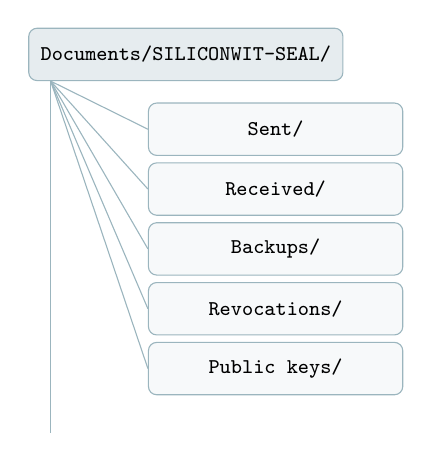
\begin{tikzpicture}[scale=0.95, transform shape]
        \node[folder, minimum width=4.2cm, fill=swSlate!15, font=\footnotesize\bfseries\ttfamily] (root) at (0, 3.0) {Documents/SILICONWIT-SEAL/};
        \node[folder, minimum width=3.4cm] (sent) at (1.2, 2.0) {Sent/};
        \node[folder, minimum width=3.4cm] (recv) at (1.2, 1.2) {Received/};
        \node[folder, minimum width=3.4cm] (back) at (1.2, 0.4) {Backups/};
        \node[folder, minimum width=3.4cm] (revo) at (1.2, -0.4) {Revocations/};
        \node[folder, minimum width=3.4cm] (pubk) at (1.2, -1.2) {Public keys/};
        \draw[swSlate!60] (root.south west) ++(0.3, 0) -- ++(0, -4.7) coordinate (treebase);
        \foreach \n in {sent, recv, back, revo, pubk} {
          \draw[swSlate!60] ($(root.south west) + (0.3, 0)$ |- \n.west) -- (\n.west);
        }
      \end{tikzpicture}
    \end{column}
    \begin{column}{0.42\textwidth}
      \footnotesize
      \begin{itemize}
        \item \textbf{Sent/} encrypted bundles you sealed
        \item \textbf{Received/} decrypted contents, one subfolder per bundle
        \item \textbf{Backups/} private-key backup files (\texttt{.asc})
        \item \textbf{Revocations/} revocation certificates (\texttt{.asc})
        \item \textbf{Public keys/} your exported public keys (\texttt{.asc})
      \end{itemize}
      \vspace{0.4em}
      Change the parent folder from \textbf{Settings}, then \textbf{Files location}. Seal always creates a \texttt{SILICONWIT-SEAL} subfolder so its files never spill into your other documents.
    \end{column}
  \end{columns}
\end{frame}

% ===== Slide 12: daily use ==============================================
\begin{frame}{Daily use, in two minutes}
  \begin{columns}[T,onlytextwidth]
    \begin{column}{0.5\textwidth}
      \begin{itemize}
        \item \textbf{Send.} Drag files in, pick recipients, click \emph{Encrypt and Save}.
        \item \textbf{Receive.} Drag the \texttt{.gpg} / \texttt{.pgp} / \texttt{.asc} in, type passphrase, contents extract.
        \item \textbf{Contacts.} Paste or import \texttt{.asc} files. Mark \textbf{verified} after confirming the fingerprint over a trusted channel.
        \item \textbf{My Keys.} Re-export backups, replace a lost key, add a second identity.
      \end{itemize}
    \end{column}
    \begin{column}{0.46\textwidth}
      \centering
      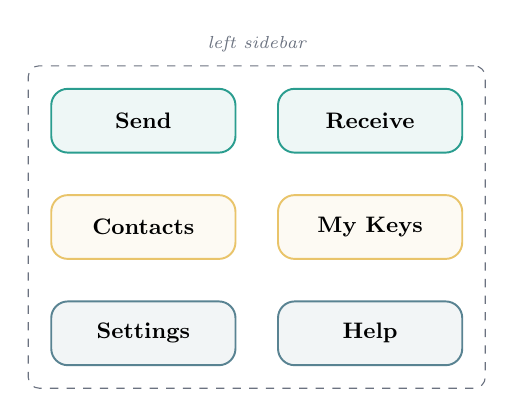
\begin{tikzpicture}[scale=0.9, transform shape]
        \node[card=swTeal, minimum width=2.6cm, minimum height=0.9cm] (send) at (-1.6, 1.5) {\textbf{Send}};
        \node[card=swTeal, minimum width=2.6cm, minimum height=0.9cm] (recv) at (1.6, 1.5) {\textbf{Receive}};
        \node[card=swAmber, minimum width=2.6cm, minimum height=0.9cm] (cont) at (-1.6, 0.0) {\textbf{Contacts}};
        \node[card=swAmber, minimum width=2.6cm, minimum height=0.9cm] (keys) at (1.6, 0.0) {\textbf{My Keys}};
        \node[card=swSlate, minimum width=2.6cm, minimum height=0.9cm] (set) at (-1.6, -1.5) {\textbf{Settings}};
        \node[card=swSlate, minimum width=2.6cm, minimum height=0.9cm] (help) at (1.6, -1.5) {\textbf{Help}};
        \begin{scope}[on background layer]
          \node[draw=swMute, dashed, rounded corners, fit=(send) (recv) (cont) (keys) (set) (help), inner sep=8pt] (nav) {};
        \end{scope}
        \node[legend, above=2pt of nav] {left sidebar};
      \end{tikzpicture}
    \end{column}
  \end{columns}
\end{frame}

% ===== Slide 13: closing =================================================
\begin{frame}[plain]
  \vspace*{1.2cm}
  \begin{center}
    {\color{swTealDark}\rule{3em}{4pt}}\\[1.0em]
    {\usebeamerfont{title}\usebeamercolor[fg]{title}You are ready.}\\[1.0em]
    {\usebeamerfont{subtitle}\usebeamercolor[fg]{subtitle}Drag a file in. Pick a recipient. Send.}\\[2em]
    {\small Quick start: \href{\docsurl quickstart/}{siliconwit.github.io/siwit-seal-releases/quickstart}}\\[0.4em]
    {\small Tour: \href{\docsurl using/}{siliconwit.github.io/siwit-seal-releases/using}}\\[0.4em]
    {\small Releases: \href{\releasesurl}{github.com/SiliconWit/siwit-seal-releases/releases}}
  \end{center}
\end{frame}

\end{document}
